\subsection{Markov Models}
\paragraph{Definition}
It \tB{assumes that $X_{t}$ captures all the relevant information for predicting the future}.
If we assume discrete time steps the \tB{joint distribution} is:
\begin{center}
    \fr{$\prob{X_{1:T}} = \prob{X_{1}}\prd{t=2}{T}\prob{X_{t}|X_{t-1}}$}
\end{center}
\uB{if the transition function $\prob{X_{t}|X_{t-1}}$ is independent of time then the chain is called
\emph{homogeneous}, \emph{stationary} or \emph{time-invariant}}.\\
This assumption allows us to model an arbitrary of variables using a fixed number of parameters, such
models are called \tB{\textbf{stochastic process}}.
\paragraph{Assumptions}
\tB{$x_{t+1} \perp x_{1:t-1}|x_{t}$, meaning the future is independent of the past 
given the present}, is called the \emph{first order Markov assumption.}

\paragraph{Transition matrix}
\uB{When $X_{t}$ is discrete} the conditional distribution $\prob{X_{t}|X_{t-1}}$ can be written as 
$K\times K$ matrix known as \tB{\textbf{transition matrix} $\bm{A}$, where $A_{ij} = \prob{X_{t}=j|
X_{t-1}=i}$ being the probability of going from state $i$ to $j$}. Each row of the matrix sums to one
\tB{$\Sigma_{j}A_{ij}=1$} so it is called \emph{stochastic matrix}.
\begin{figure}[H]
    \begin{center}
        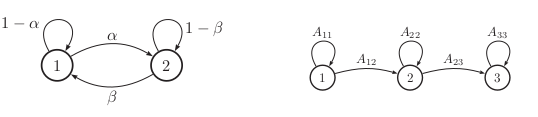
\includegraphics[width=.5\textwidth]{./chapters/2_statistics/07_hidden_markov_models/1_images/1_state_transition_diagrams.png}
    \end{center}
    \caption{State transition diagrams for, 2-state chain and 3-state chain.}
    \label{fig:1_state_transition_diagrams}
\end{figure}
The $n$-step transition matrix $\bm{A}(n)$ is defined as \tB{$\bm{A}_{ij}(n)=\prob{X_{t+n}=j|
X_{t}=i}$}\\
For a steps $m+n$ , \tB{$\bm{A}(m+n) = \bm{A}(m) + \bm{A}(n)$}

\paragraph{Application}
\begin{itemize}
    \item Language modeling
    \begin{itemize}
        \item Sentence completion
        \item Data compression
        \item Text classification
        \item Automatic essay writing
    \end{itemize}
\end{itemize}
\paragraph{MLE for Markov language models}
The \uB{probability of any particular sequence of length T} is given by:
\begin{center}
    $
\prob{x_{1:T}|\bm{\theta}} = \pi(x_{1})\prd{t=2}{T}A(x_{t-1},x_{t}) = 
\prd{i=1}{K}\pi_{i}^{\mathbbm{1}_{\{x_{1}=i\}}}\prd{t=2}{T}\prd{j=1}{K}\prd{i=1}{K}
A_{ij}^{\mathbbm{1}_{\{x_{t}=j,x_{t-1}=i\}}}
$
\end{center}

Then the log-likelihood of a set of sequences $\mathcal{D}=\left\{\bm{x}_{i}\right\}_{1\leq i\leq n}$
:
\begin{center}
    \fr{$\log\left(\prob{\mathcal{D}|\bm{\theta}}\right) = \su{n=1}{N}\log\left(\prob{\bm{x}_{n}|\bm{
            \theta}}\right) = \su{i}{}N_{i}^{(1)}\log(\pi_{i}) + \su{i}{}\su{j}{}N_{ij}\log(a_{ij})$}
\end{center}
where $\hat{\pi}_{i}=\dfrac{N_{i}^{(1)}}{\su{i'}{K}N_{i'}^{(1)}}$ and 
$\hat{a}_{ij}=\dfrac{N_{ij}}{\su{j'}{K}N_{ij'}}$

\paragraph{Stationary distribution of a Markov chain}
We can interpret Markov models as stochastic dynamical systems, where we hop from one state to 
another at each time step, we are then often interested in the \tB{long term 
distribution over states, called \emph{stationary distribution}}.\\
Considering the transition matrix $\bm{A}$ defined by $\bm{A}_{ij}=\prob{X_{t}=j|X_{t-1}=i}$ and 
the probability to be at a given state at time t $\bm{\pi}$ defined by $\pi_{t}(j)=\prob{X_{t}=j}$.\\
\tB{If we ever reach a stage where $\bm{\pi}=\bm{\pi}\bm{A}$ then we have reached the \emph{
stationary distribution}}.\\



\subsection{Hidden Markov Models}
\paragraph{Definition}
It consists of a discrete-time, \tB{discrete-state Markov chain, with hidden states} 
$z_{t}\in\inter{1}{K}$.\\
The corresponding joint distribution has the form:
\begin{center}
    \fr{$\prob{\bm{z}_{1:T}, \bm{x}_{1:T}} = \prob{\bm{z}_{1:T}}
\prob{\bm{x}_{1:T}|\bm{z}_{1:T}}=
\left[\prob{z_{1}}\prd{t=2}{T}\prob{z_{t}|z_{t-1}}\right]\prd{t=1}{T}\prob{\bm{x}_{t}|z_{t}}$}   
\end{center}

It's common to have for:
\begin{itemize}
    \item \emph{discrete} observations: $\prob{\bm{x}_{t}=l|z_{t}=k,\bm{\theta}} = \text{\emph{Beta}}
        (k,l)$
    \item \emph{continuous} observations: $\prob{\bm{x}_{t}|z_{t}=k,\bm{\theta}} = \mathcal{N}(\bm{x}
        _{t}|\bm{\mu}_{k},\bm{\Sigma}_{k})$
\end{itemize}

\paragraph{Strengths}
\begin{itemize}
    \item can represent long-range dependencies between observations compared to Markov models
    \item useful for time series prediction
    \item can define class-conditional densities inside a generative classifier
\end{itemize}

\paragraph{Examples}
\begin{itemize}
    \item Automatic speech recognition: $\bm{x}_{t}$ represents features extracted from the speech 
        signals and $z_{t}$ represents the word that is being spoken
    \item Activity recognition: $\bm{x}_{t}$ represents feature extracted from a video frame and 
        $z_{t}$ is the class of activity the person is engaged (running, waking, sitting)
\end{itemize}

\paragraph{Types of inferences}
\begin{itemize}
    \item \textbf{Filtering}: \tB{computing the \emph{belief state} $\prob{z_{t}|
        \bm{x}_{1:t}}$} \tR{online or recursively as the data streams in}. The name
        \uB{"filtering" is due to the noise reduction induced with the hidden state 
        estimating}  using the current $\prob{z_{t}|\bm{x}_{t}}$
    \item \textbf{Smoothing}: \tB{computing $\prob{z_{t}|\bm{x}_{1:T}}$} \tR{offline}
        given all the evidence 
    \item \textbf{Fixed Lag Smoothing}: \tB{computing $\prob{z_{t-l}|\bm{x}_{1:t}}$}
        that is an \uB{interesting compromise between online and offline} estimation.
        It provides better performance than filtering but incurs a slight delay.
        \uB{Changing the lag size, one can trade off \emph{accuracy} vs \emph{delay}}
    \item \textbf{Prediction}: \tB{computing $\prob{z_{t+h}|\bm{x}_{1:t}}$} where
        \tR{$h>0$ is called the \emph{prediction horizon}}. For example $h=2$ implies 
        $\prob{z_{t+2} |\bm{x}_{1:t}} = \su{z_{t+1}}{}\su{z_{t}}{}\prob{z_{t+2}|
        z_{t+1}} \prob{z_{t+1}|z_{t}} \prob{z_{t}|\bm{x}_{1:t}}$
    \item \textbf{MAP estimation}: \tB{computing $\displaystyle\argmin_{(\bm{z}_{k})_{
                1\leq k\leq t}}$} which is most probable state sequence.
    \item \textbf{Posterior samples}: if there is more that one plausible 
        interpretation of the data, it can be useful to sample from the posterior 
        $\bm{z}_{1:t} \hookrightarrow \prob{\bm{z}_{1:t}|\bm{x}_{1:t}}$
    \item \textbf{Probability of the evidence}: \tB{compute $\prob{\bm{x}_{1:t}}=
        \su{\bm{z}_{1:t}}{}\prob{\bm{z}_{1:t}, \bm{x}_{1:t}}$} meaning summing up 
        over all hidden paths. Can be used to classify sequences for model-based 
        clustering, anomaly detection.
\end{itemize}

\subsection{Inference HMMs}
\paragraph{The forward algorithm}
\subparagraph{Purpose} recursively \tB{computing the filtered marginals}: for $j\in\inter{1}{K}~
\prob{z_{t}=j|\bm{x}_{1:t}}$ in a hidden Markov model.
\subparagraph{Steps}
\begin{enumerate}
    \item \emph{Prediction step}: computing the \emph{one-step-ahead predictive 
        density} acting as the new prior for $t$:\\ $\prob{z_{t}=j|\bm{x}_{1:t-1}} =
        \su{i}{} \prob{z_{t}=j| z_{t-1}=i}\prob{z_{t-1}=i|\bm{x}_{1:t-1}}$
    \item \emph{Update step}: we absorb the observed data from $t$ using Bayes rule:\\
        $\alpha_{t}(j) \triangleq \prob{z_{t}=j| \bm{x}_{1:t}} = \prob{z_{
            t}=j| \bm{x}_{t}, \bm{x}_{1:t-1}} = \frac{1}{Z_{t}}\prob{\bm{x}_{
        t}|z_{t}=j} \prob{z_{t}=j|\bm{x}_{1:t-1}}$ 
        where  the normalization constant is $Z_{t} \triangleq \prob{\bm{x}_{t}|
        \bm{x}_{1:t-1}}=\su{j}{}\prob{\bm{x}_{t}|z_{t}=j}\prob{z_{t}=j|\bm{x}_{1:t-1}}$\\
        Hint: consider $\bm{x}_{t}\perp\bm{x}_{1:t-1}|z_{t}$
\end{enumerate}
The distribution \tB{$\prob{z_{t}|\bm{x}_{1:t}}$ is called the (filtered) belief state at time t},
it is a vector of $K$ numbers denoted $\bm{\alpha}_{t}$
Considering $\odot$ being the \emph{Hadamard product} representing element-wise vector 
multiplication.
\begin{center}
    \fr{$\bm{\alpha}_{t} \propto \bm{\psi}_{t} \odot \bm{\Psi}^{T}\bm{\alpha}_{t-1}$}
\end{center}
where $\psi_{t}(j) = \prob{\bm{x}_{t}|z_{t}=j}$ being the local evidence at time $t$ and $\bm{\Psi}(
i,j)=\prob{z_{t}=j|z_{t-1}=i}$ is the transition matrix.

\paragraph{Forwards-Backwards algorithm}
\subparagraph{Purpose}
\tB{Computing smoothed marginals $\prob{z_{t}=j|\bm{x}_{1:T}}$} using offline inference.
\subparagraph{Basic idea}
The key decompositions relies on the fact that \tB{we can break the chain into two parts: the \emph{
past} and the \emph{future} by conditioning on $z_{t}$}\\
Let \tB{$\alpha_{t}(j)\triangleq\prob{z_{t}=j|\bm{x}_{1:t}}$} be the filtered belief state as before.
Define as well \tB{$\beta_{t}(j)\triangleq \prob{\bm{x}_{t+1:T}|z_{t}=j}$} being the \uB{conditional 
likelihood of the future evidence given that the hidden state at time $t$ is $j$.}\\
Finally define \tB{$\gamma_{t}(j) \triangleq \prob{z_{t}=j|\bm{x}_{1:T}}$ as the desired smoothed
posterior marginal}.\\
We previously described how to recursively compute the $\alpha$'s in a \emph{left-to-right} fashion.
We now describe how to recursively compute the $\beta$'s in a \emph{right-to-left} fashion.
\begin{align*}
    \beta_{t-1}(i) &= \prob{\bm{x}_{t:T}|z_{t-1}=i}\\
                   &= \su{j}{}\prob{z_{t}=j,\bm{x}_{t},\bm{x}_{t+1:T}|z_{t-1}=i}\\
                   &= \su{j}{}\prob{\bm{x}_{t+1:T}|z_{t}=j, \cancel{z_{t-1}=i}, \cancel{\bm{x}_{t}}}
                   \prob{z_{t}=j,\bm{x}_{t}|z_{t-1}=i}\\
                   &= \su{j}{}\prob{\bm{x}_{t+1:T},z_{t}=j}\prob{\bm{x}_{t}|z_{t}=j,
                       \cancel{z_{t-1}=i}}\prob{z_{t}=j|z_{t-1}=i}\\
                   &= \su{j}{}\beta_{t}(j)\psi_{t}(j)\Psi(i,j)
\end{align*}
In matrix-vector form: \tB{$\bm{\beta}=\bm{\Psi}\left(\bm{\psi}_{t}\odot\bm{\beta}_{t}\right)$}
We can think of this algorithm as passing "messages" from left to right and then from right to
left and then combining them at each node.
\subparagraph{Complexity}
It takes $O(K^{2}T)$ time since at each step we perform a $K\times K$\\
We can think of this algorithm as \uB{passing "messages" from left to right and then from right to 
left, and then combining them at each node}. Finally 
\begin{center}
    \fr{$\gamma_{t}(j) \propto \alpha_{t}(j) \beta_{t}(j)$}
\end{center}


\paragraph{The Viterbi Algorithm}
\subparagraph{Purpose}
\tB{Compute the most probable sequence of states} in a chain-structured graphical model: \tB{$\bm{z}^{*}=
\displaystyle\argmax_{\bm{z}_{1:T}}\prob{\bm{z}_{1:T}|\bm{x}_{1:T}}$}.\\
This is equivalent to computing a shortest path through \textit{trellis diagram} where the nodes are 
possible states at each time step and the node and edge weights are log probabilities.
\begin{figure}[H]
    \begin{center}
        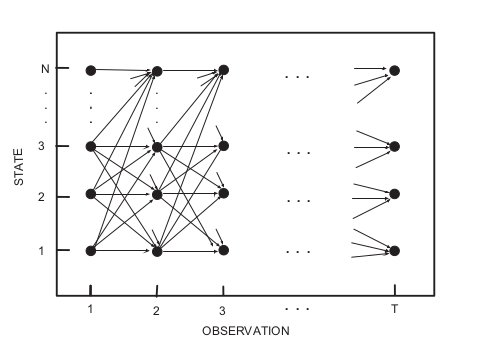
\includegraphics[width=.5\textwidth]{chapters/2_statistics/07_hidden_markov_models/2_images/2_trellis_diagram.png}
    \end{center}
    \caption{Trellis diagram: states vs time for a Markov chain.}
    \label{fig:2_trellis_diagram}
\end{figure}
\paragraph{MAP vs MPE}
The (\emph{jointly}) most probable sequence of states: $\bm{z}^{*}$ is not necessarily the same as 
the sequence of (\emph{marginally}) most probable states, \emph{Maximize of the Posterior Marginals}
(MPM): $\hat{\bm{z}}=\left(\displaystyle\argmax_{
z} \prob{z|\bm{x}_{1:T}}\right)_{z_{1}\leq z\leq z_{T}}$.\\
In one hand \tB{the joint MAP estimate is that is always globally consistent} on the other hand
the \tB{MPM estimate can be more robust}
\subparagraph{Detail of the algorithm}
Although is tempting to implement Viterbi by replacing the sum-operator with max-operator in the
forward-backwards, it can lead to incorrect results if there are multiple equally probably joint
assignments. Therefore \tB{Viterbi uses max-product in the forward pass and a traceback procedure in 
the backwards pass}.\\
Let's define the \uB{probability of ending up in state $j$ at time $t$ given that we take the most
probable path}:
\begin{center}
    \fr{$\delta_{t}(j)\triangleq \displaystyle\max_{\bm{z}_{1:t-1}}\prob{\bm{z}_{1:t-1}, z_{t}=j|
    \bm{x}_{1:t}}$}
\end{center}
The key insight is that \tB{the most probable path to state $j$ at time $t$ must consist of the most
probable path to some other state $i$ at time $t-1$, followed by a transition from $i$ to $j$}.
\begin{enumerate}
    \item Hence $\delta_{t}(j) = \displaystyle\max_{i}\delta_{t-i}(i)\Psi(i,j)\psi_{t}(j)$
    \item \uB{Keeping track of the most likely previous state} for each possible state that we end 
        up: $a_{t}(j) = \displaystyle\argmax_{i}\delta_{t-1}(i)\Psi(i,j)\psi_{t}(j)$. It tells us the
        \uB{most likely previous state on the most probable path to $z_{t}=j$}.
    \item initialize $\delta_{1}(j)=\pi_{j}\psi_{1}(j)$
    \item compute the most probable final state $z_{T}^{*}=\displaystyle\argmax_{j}\delta_{T}(j)$
    \item using traceback we can compute the most probable sequence of states: $z_{t}^{*}=a_{t+1}(
        z^{*}_{t+1})$
\end{enumerate}

\subparagraph{Complexity}
It is $O(K^{2}T)$

\paragraph{Forwards filtering, backwards sampling}
\subparagraph{Purpose}
Sample paths from posterior: $\bm{z}^{s}_{1:T} \hookrightarrow \prob{\bm{z}_{1:T}|\bm{x}_{1:T}}$
\uB{Without being obliged to perform forward-backwards pass} and then an additional 
forward sampling pass.
\subparagraph{Steps}
The key insight is that to do forward pass and then perform sampling in the backward pass we can
write the joint from right to left using
$\prob{\bm{z}_{1:T}|\bm{x}_{1:T}} = \prob{z_{T}|\bm{x}_{1:T}
}\prd{t=T-1}{1}\prob{z_{t}|z_{t+1},\bm{x}_{1:T}}$\\
Then we can sample $z_{t}$ given future sampled states using:\\
$z^{s}_{t} \hookrightarrow\prob{z_{t}|z_{t+1:T},\bm{x}_{1:T}} = \prob{z_{t}|z_{t+1},\cancel{\bm{z}_{
t+2:T}}, \cancel{\bm{x}_{t+1:T}}} =  \prob{z_{t+1}|z_{t+1}^{s},\bm{x}_{1:t}}$\\

The sampling distribution is given by:
\begin{align*}
    \prob{z_{t}=i|z_{t+1}=j,\bm{x}_{1:t}}
    &= \prob{z_{t}|z_{t+1},\bm{x}_{1:t},\cancel{\bm{x}_{t+1}}}\\
    &= \dfrac{\prob{z_{t+1},z_{t}|\bm{x}_{1:t+1}}}{\prob{z_{t+1}|\bm{x}_{1:t+1}}}\\
    &\propto \dfrac{\prob{\bm{x}_{t+1}|z_{t+1},\cancel{z_{t}},\cancel{\bm{x}_{1:t}}}\prob{z_{t+1},
            z_{t}|\bm{x}_{1:t}}}{\prob{z_{t+1},z_{t}|\bm{x}_{1:t+1}}}\\
    &= \dfrac{\prob{\bm{x}_{t+1}|z_{t+1}}\prob{z_{t+1}|z_{t},\cancel{\bm{x}_{1:t}}}\prob{z_{t}|
    \bm{x}_{1:t}}}{\prob{z_{t+1},z_{t}|\bm{x}_{1:t+1}}}\\
    &= \dfrac{\phi_{t+1}(j)\psi(i,j)\alpha_{t}(i)}{\alpha_{t+1}(j)}
\end{align*}

\subsection{Learning for HMMs}
We want to \tB{estimate the parameters $\bm{\theta}=(\bm{\pi}, \bm{A}, \bm{B})$} where $\pi(i)=\prob{
z_{i}=i}$ is the initial state distribution, $\bm{A}(i,j)=\prob{z_{t}=j|z_{t-1}=i}$ the transition
matrix and \uB{$\bm{B}$ the parameters of the class-conditional densities $\prob{\bm{x}_{t}|z_{t}=j}$
}
\paragraph{Training with fully observed data}
If we observe the hidden state sequences, we cna compute the MLEs for $\bm{A}$ and $\bm{\pi}$ 
exactly. \\
In using a conjugate prior we can easily compute the posterior.\\
The details on how to \tB{estimate $B$ depend on the form of the observation model}.

\paragraph{EM for HMMs (Baum-Welch Algorithm)}
If $z_{t}$ are not observed we are in a situation analogous to fitting a mixture model.
The most common approach is to \tB{use EM algorithm to find the MLE or MAP parameters}.

\subparagraph{E step}
It is straightforward to show that the expected complete data log likelihood is given by:
\begin{center}
    $Q(\bm{\theta},\bm{\theta}^{old}) = \su{k=1}{K}\E{N^{1}_{k}}\log(\pi_{k}) \su{j=1}{K}\su{k=1}{K}
        \E{N_{jk}}\log(A_{jk}) + \su{i=1}{N}\su{t=1}{T_{i}}\su{k=1}{K}\prob{z_{t}=k|\bm{x}_{i},
        \bm{\theta}^{old}}\log\left(\prob{\bm{x}_{i}|\phi_{k}}\right)$
\end{center}
where 
$\begin{cases}
    \E{N^{1}_{k}} &= \su{i=1}{N}\prob{z_{i1}=k|\bm{x}_{i},\bm{\theta}^{old}} \\
    \E{N_{jk}} &= \su{i=1}{N}\su{t=1}{T_{i}}\prob{z_{i,t-1}=j,z_{i,t}=k|\bm{x}_{i},\bm{\theta}^{
    old}} \\
            \E{N_{j}} &= \su{i=1}{N}\su{t=1}{T_{i}}\prob{z_{i,t}=k|\bm{x}_{i},\bm{\theta}^{old}}
\end{cases}$
These expected sufficient statistics can be computed by running the forward-backward algorithm on 
each sequence.\\
In particular, this algorithm computes the following smoothed node and edge marginals:\\
$\begin{cases}
    \gamma_{i,t}(j) \triangleq \prob{z_{t}=j|\bm{x}_{i,1:T_{i}},\bm{\theta}} \\
    \xi_{i,t}(j,k) \triangleq \prob{z_{t-1}=j,z_{t}=k|\bm{x}_{i,1:T},\bm{\theta}}
\end{cases}$

\subparagraph{M step}
From results in mixture of Multinoulli:
$\hat{A}_{jk} = \dfrac{\E{N_{k}}}{\su{k'}{}\E{N_{jk'}}}, \hat{\pi}_{k}=\dfrac{\E{N^{1}_{k}}}{N}$\\
For a Multinoulli observation model the expected sufficient statistics are:
$\E{M_{jl}} = \su{i=1}{N}\su{t=1}{T_{i}}\gamma_{i,t}(j)\mathbbm{1}_{\{x_{i,t}=l\}} = 
\su{i=1}{N}\su{t:x_{i,t}=l}\gamma_{i,t}(j)$.\\
The M step has the form $\hat{B}_{jl} = \dfrac{\E{M_{jl}}}{\E{N_{j}}}$.\\
For a Gaussian observation model:
$\begin{cases}
    \E{\overline{x}_{k}} = \su{i=1}{N}\su{t=1}{T_{i}}\gamma_{i,t}(k)\bm{x}_{i,t} \\
    \E{(\overline{x}\overline{x})^{T}_{k}} = \su{i=1}{N}\su{t=1}{T_{i}}\gamma_{i,t}(k)\bm{x}_{i,t}
    \bm{x}^{T}_{i,t}
\end{cases}$

The $M$ step becomes :

$\begin{cases}
    \hat{\bm{\mu}}_{k} = \dfrac{\E{\overline{\bm{x}}_{k}}}{\E{N_{k}}} \\
    \hat{\bm{\Sigma}}_{k} = \dfrac{\E{(\overline{x}\overline{x})^{T}_{k}} - \E{N_{k}}\hat{\bm{\mu}}_
    {k} \bm{{\mu}}^{T}_{k}}{\E{N_{k}}}
\end{cases}$

\paragraph{Bayesian methods for 'fitting' HMMs}
We can use variational Bayes EM method, the \uB{E step uses forwards-backwards but where we plug in
the posterior mean parameters instead of the MAP estimates}. The \uB{M step updates the parameters o
the conjugate posteriors instead of updating the parameters themselves}.

\paragraph{Model selection}
\subparagraph{Choosing the number of hidden states}
\begin{itemize}
    \item using grid-search over range of $K$'s 
    \item Variational Bayes to "extinguish" unwanted components
    \item Use an "infinite HMM" which is based on the hierarchical Dirichlet process
\end{itemize}

